\documentclass[12pt, a4paper]{article}

\usepackage[T1]{fontenc}
\usepackage[utf8]{inputenc}
\usepackage[polish]{babel}
\usepackage[margin=2cm]{geometry}
\usepackage{indentfirst}
\usepackage{amsmath}
\usepackage{enumitem}
\usepackage{graphicx}
\usepackage{textgreek}
\usepackage{float}

\begin{document}
	
	\begin{center}
		\Huge \textbf{Analiza porównawcza wpływu kursu przygotowawczego na wyniki } \\[0.5em]
		\large Sprawozdanie 1 \\[1.5em]
		\Large Martyna Pacyna 287440 \\ Lena Rojecka 287460
	\end{center}


\section{Wstęp}
	Analizowany zbiór danych pochodzi z platformy Kaggle i dotyczy wyników egzaminacyjnych uczniów szkół średnich z trzech głównych przedmiotów: matematyki (math score), czytania (reading score) oraz pisania (writing score). Zbiór składa się z 1000 obserwacji, z których każda opisuje pojedynczego ucznia za pomocą 8 cech. Jest to zestaw danych stworzony głównie w celach edukacyjnych. Głównym celem niniejszego sprawozdania jest przeprowadzenie analizy porównawczej wyników egzaminacyjnych w dwóch grupach uczniów: tych, którzy odbyli kurs przygotowawczy, oraz tych, którzy go nie posiadali. 
	
\section{Analiza rozkładów przy pomocy metryk statystycznych}
%miary statystyczne
	Średnia arytmetyczna. Wzór: $\bar{x} = \frac{1}{n} \sum_{i = 1}^{n} x_{i}.$ \\ Ta średnia to średni wynik w grupie. Jeśli $\bar{x}$ dla grupy po kursie będzie większa niż dla grupy bez kursu, to kurs będzie podnosił ogólny poziom wiedzy studenta. \\ 
	Mediana. \\ \\
%miary położenia
	Odchylenie standardowe. Wzór: $s = \sqrt{\dfrac{\sum (x_{i} - \bar{x})^2}{n - 1}}.$ \\ \\
%miary kształtu
	Skośność. \\
	Kurtoza. \\ \\
\section{Prezentacja rozkładów na wykresach}
\begin{figure}[h!]
	\centering
	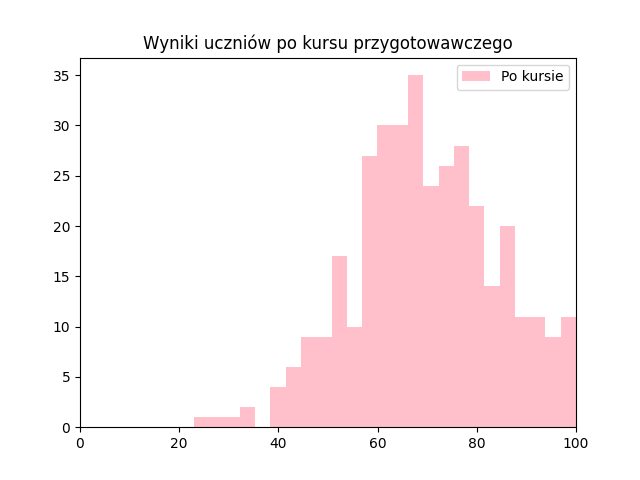
\includegraphics[width=0.4\textwidth]{po_kursie_math.png} 
	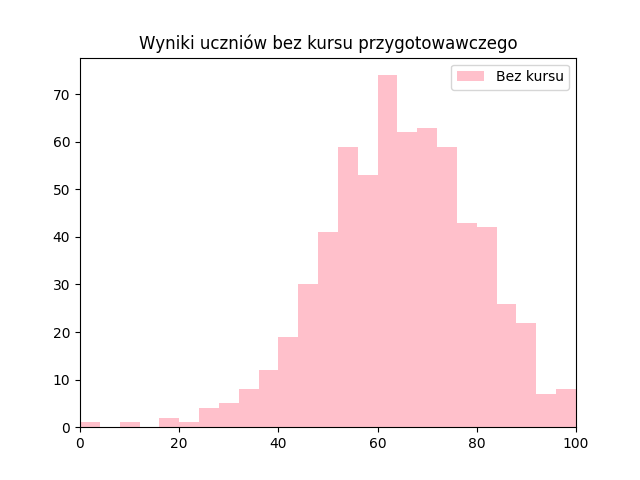
\includegraphics[width=0.4\textwidth]{bez_kursu_math.png} 
\end{figure}

\begin{figure}[h!]
	\centering
	
\includegraphics[width=0.4\textwidth]{z_z_norm.png} 
	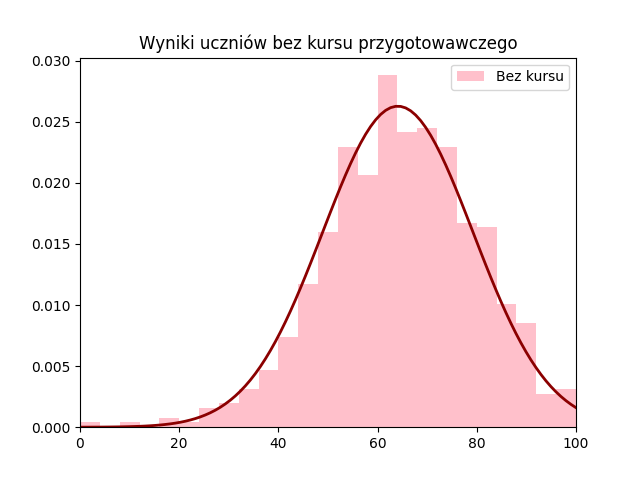
\includegraphics[width=0.4\textwidth]{bez_z_norm.png} 
\end{figure}

\begin{figure}[h!]
	\centering
	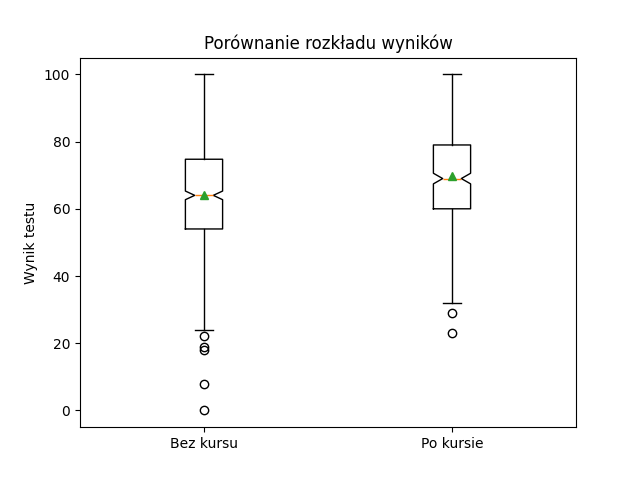
\includegraphics[width=0.4\textwidth]{boxploty.png} 
\end{figure}
\section{Wnioski}
\end{document}